	\documentclass[10pt]{IEEEtran}
\pdfoutput=1

\usepackage{graphicx}
\graphicspath{{figures/}}
\usepackage{hyperref}
\usepackage[utf8]{inputenc}
\usepackage{listings}
\usepackage[table]{xcolor}
\usepackage{pdfpages}
\usepackage[justification=centering]{caption}
\usepackage{float}

\hypersetup{colorlinks=true,citecolor=[rgb]{0,0.4,0}}


\title{Analysis of the susceptibility of Twitter users}
\author{Søren Howe Gersager, Anders Lønberg Rahbek}

\begin{document}
\maketitle

\begin{abstract}
This report is the result of the final project in DTU course 02805: Social Graph and Interactions. The course subject was analyzing social networks using Twitter bots and the relation and interaction between bot and human. \\
This final project tries to look into what makes a human subsceptible to follow a Twitter bot.
\end{abstract}

\section{Introduction}
The purpose of DTU course 02805: Social Graph and Interactions is to make the students familiar with social networks and use network theory, natural language processing, datamining and machine learning to analyze these networks. All of the students were given the task of creating a Twitter bot with the purpose of "infiltrating" Twitter and gain followers. To gain followers the bot should try to imitate being a human user. As the followers and "Twitter presence" of the bot grew, it was used to try to influence the people of San Francisco through interventions. Interventions are created by letting all the bots tweet, retweet and favorite using a predetermined hashtag and in this way generate interactions from Twitter users. For the course, we created the bot JackBoHorseMan\cite{twitterprofile}, a 30-something male from Chicago, who loves animals, indie music, travelling and the Bulls.

\section{Implementation}
\subsection{Circadian Rhythm}
By using the job-scheduler cron we were able to make the bot interact with Twitter in a simulated circadian rhythm between 8:00 to 22:00 PST (San Francisco Timezone), with a random delay of 0 to 15 minutes included. This was done to make the bot appear more human.
The implementations in the next subsections all operate only in the circadian rhythm specified here.

\subsection{Tweeting}
The bot tweeted using two principles:
\begin{itemize}
\item Personal tweets: we created a list of predetermined tweets that the bot could select tweets from, communicating every-day situations as working late or waiting for the weekend or being tired on a monday that human users might relate or respond to.
\item Event tweets: The bot scraped the website of San Francisco Weekly and collected upcoming events like concerts, book readings, plays and tweeted about them in a fitting context randomly chosen from a list of fitting nouns and adjectives like "attending", "going to" and "rocking", "chill".
\end{itemize}
\subsection{Reciprocal Following}
Once a day we followed new twitter users based on two principles:
\begin{itemize}
\item Followback query: we performed a search for new users using a query on "followback", and followed them hoping they would follow us back. This principle was to artificially boost the number of followers and followed of the bot and thus look more attractive from a social point of view to potential human users.
\item Human query: we performed a search for new users based in San Francisco and followed them, the followers generated this way creates data for the later analysis of subsceptibility.\\
 If the users we followed didn't follow us back within 24 hours, we unfollowed them to make sure the ratio of followers to followed was kept as low as possible as a high ratio might arouse suspicion that our account is a bot account.
\end{itemize}
\subsection{Retweeting}
Once a day we retweeted content twice based on two different principles:
\begin{itemize}
\item Popularity: simply the most popular tweet based on number of retweets the bot had seen within the last 24 hours.
\item "Goodness": We trained a Naive Bayes classifier to be able to predict "good" tweets where the "goodness" criteria was that the tweet had 10 or more retweets. We used the following attributes: number of followers of the twitter account, age of the twitter account, number of links in the tweet, number of words in the tweet, and number of hashtags in the tweet. We divided the tweets into two data sets and used 2-fold cross validation on them. By doing this we could predict which tweets had the potential to be "good" retweeted tweets.
\end{itemize}

\subsection{Twitter Profile Variation}
The bot updated the Twitter profile every third day with a new profile banner based on a Google Image search, finding 50 on topics: horses, animals, indie, maldives, chicago bulls, san francisco monuments. This was done to make the bot appear more human as well as to pique the interest of potential followers.

\section{Interventions}
In the last part of the course, the whole class participated in "interventions" through their bots, Events where the bots collectively posted, retweeted and favorited content about a specific subject. These interventions hyped some predifined hashtags through two original tweets per day every Mondays, Wednesdays and Fridays plus at Thanksgiving. \\
Out strategy was to have the bot do it autonomously so we didn't have to intervene. \\

We wrote all the original tweets and their hashtags in a semicolon seperated text-file where the specified date was the first element - then the two tweets. Our bot could then read the file, make a dictionary with the dates as keys and the two tweets as values. \\

The window where the bot posted the two tweets was between 9am and 1pm San Francisco time. We add randomness to the time where the posts of the tweets would occur, by using random.sleep before both of the tweets.\\
Two cron jobs ensured that the bot did every Mondays, Wednesdays and Fridays plus thanksgiving.\\\\\\\\


\begin{figure}[H]
  \centering
 \hspace*{-1.8cm}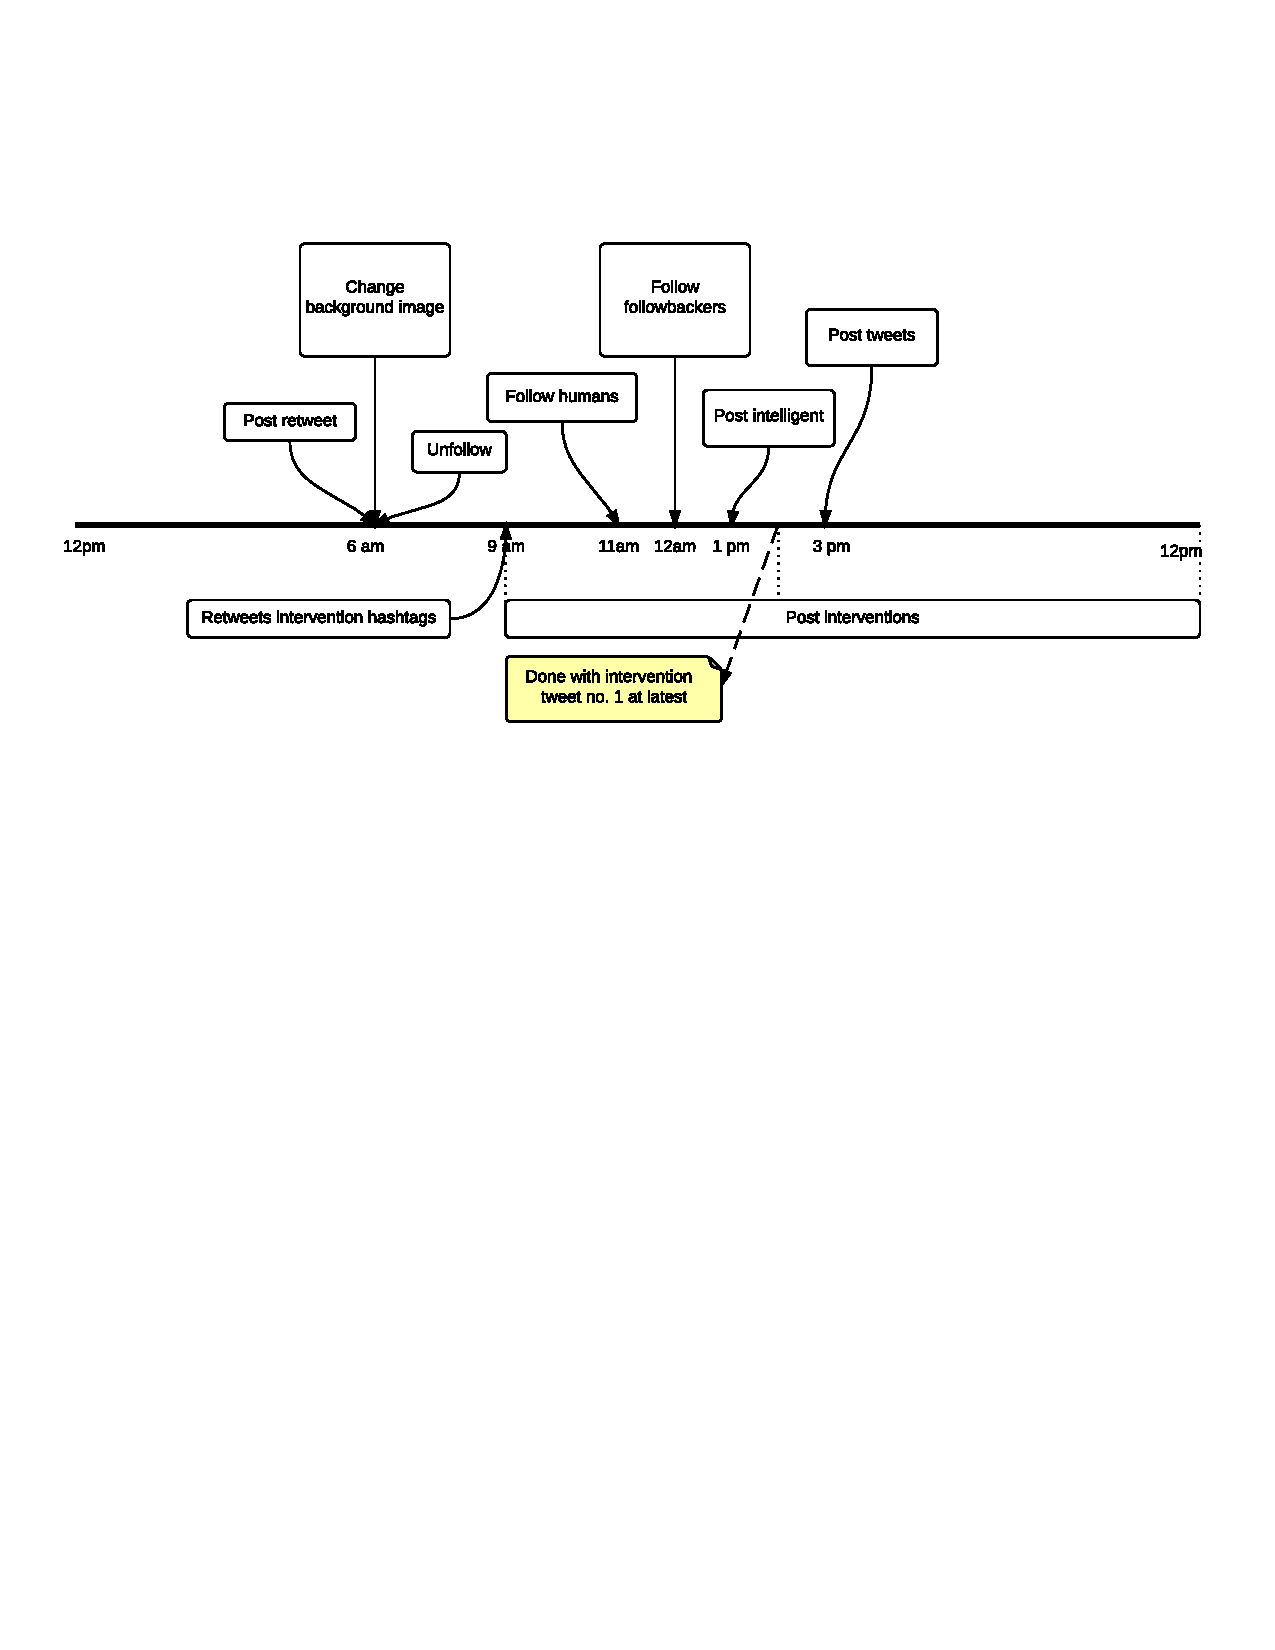
\includegraphics[trim=0.5cm 15cm 0.5cm 4cm,width=4.3in]{intervention_timeline}
  \caption{Timeline over out bots activities}
  \label{fig:bot}
\end{figure}

\section{Susceptibility analysis}
\subsection{User groups}
The foundation of our analysis consists of two groups: the susceptible and non-susceptible twitter users. The susceptible users group consists of 488 users, 487 of which allowed us to see their information and tweets. The non-susceptible users group consists of 1186 users, 1183 of which allowed us to see their information and tweets.

For performing analysis on tweets, 26 users from the non-susceptible group did not have any tweets, which shrunk the group down to 1160 when analysing tweets. Just one of the users in the susceptible group did not have any tweets, which gives us a group size of 487 tweets.
We will analyze the following: Age of twitter account, number of followers, number of followed, number of tweets, average links of tweets, number of hashtags, tweets in comparison to retweets.
\\
NLP:
sentiment analysis, one group more positive or negative?
difference in readability measure
\\
Machine learning:
Training a classifier with above attributes: (naive bayes, logistic regression, decision tree)
\\
Networks:
In-out degree
clustering coefficient
average path length
degree distribution
which group follow the most high-profile users (100k followers or more).

\subsection{Statistics}
This section contains statistics for each group with respect to: mean, median, standard deviation, upper quartile (75\% percentile) and lower quartile (25\% percentile).\\\\


\begin{table}[h!]
\begin{tabular}{llllll}
\textbf{}       & Mean     & Median & Std. Dev & Lower Q. & Upper Q. \\
Non-susceptible & 1458.659 & 1580   & 732.116  & 932     & 2066      \\
Susceptible     & 1204.547 & 1190   & 750.312  &  500    &   1919   
\end{tabular}
\caption{Statistics for age of account}
\end{table}

For the age of account metric, we see a difference in the means and medians for the two groups with account age for the susceptible group being slightly lower, we see a similarity in standard deviation and upper percentile, with the susceptible group having a low lower quartile.

\begin{figure}[H]
  \centering
  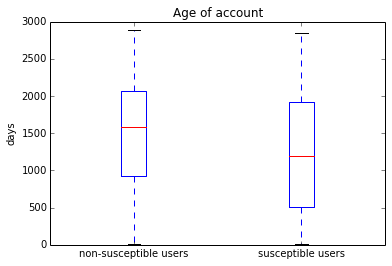
\includegraphics[width=3.0in]{age_of_account_boxplot}
  \caption{Boxplot for metric: age of account}
  \label{fig:age_boxplot}
\end{figure}
This is confirmed on the boxplot.\\\\
\begin{table}[h!]

\begin{tabular}{llllll}
\textbf{}       & Mean      & Median & Std. Dev    & Lower Q. & Upper Q. \\
Non-susceptible & 61266.122 & 1095   & 1478798.298 & 303.5    &  6013    \\
Susceptible     & 13273.042 & 1062   & 72809.619   & 388     &   1919   
\end{tabular}
\caption{Statistics for follower count}
\end{table}

Looking at the table for follower count, we see an incredibly high standard deviation and high means in comparison to medians, this is usually the result of great outliers, that seems to be mostly in the non-susceptible group.
\begin{figure}[H]
  \centering
  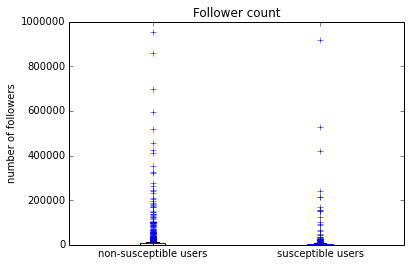
\includegraphics[width=3.0in]{follower_boxplot}
  \caption{Boxplot for metric: follower count}
  \label{fig:follower_boxplot}
\end{figure}
We see this is confirmed by looking at the boxplot where both groups have large outliers.\\\\
\begin{table}[ht!]


\begin{tabular}{llllll}
\textbf{}       & Mean      & Median & Std. Dev  & Lower Q. & Upper Q. \\
Non-susceptible & 11109.594 & 2527   & 23591.433 &  604  & 10298.5     \\
Susceptible     & 10574.918 & 2796   & 21419.868 & 709    &   10904    
\end{tabular}
\caption{Statistics for statuses count}
\end{table}
For the statuses count we see largely similar values across the board, and a high standard deviation which indicate outliers in both groups.
\begin{figure}[H]
  \centering
  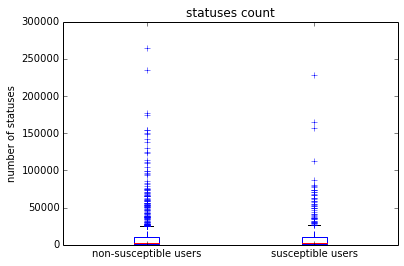
\includegraphics[width=3.0in]{statuses_count_boxplot}
  \caption{Boxplot for metric: statuses count}
  \label{fig:statuses_boxplot}
\end{figure}
This is confirmed by the boxplot where each group have outliers but seems similar.\\\\
\begin{table}[ht!]
\begin{tabular}{llllll}
\textbf{}       & Mean      & Median & Std. Dev  & Lower Q. & Upper Q. \\
Non-susceptible & 9653.624  & 1138   & 41365.673 & 431     &  3092     \\
Susceptible     & 10852.841 & 1389   & 56008.349 & 592    &   3000   
\end{tabular}
\caption{Statistics for friends count}
\end{table}

For the friends count metric they have somewhat similar values with the susceptible having a bit higher median, mean and lower quartile, with a high standard deviation indicating outliers.
\begin{figure}[H]
  \centering
  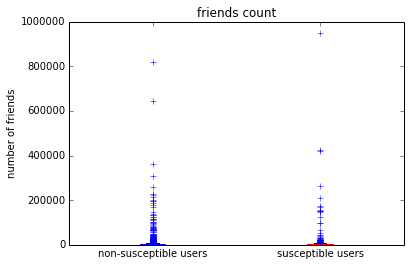
\includegraphics[width=3.0in]{friends_boxplot}
  \caption{Boxplot for metric: friends count}
  \label{fig:friends_boxplot}
\end{figure}
By looking at the boxplot we see huge outliers in friends count as well, with the median for the susceptible group being a little higher than for the non-susceptible group.\\\\
\begin{table}[ht!]
\begin{tabular}{llllll}
\textbf{}       & Mean    & Median & Std. Dev & Lower Q. & Upper Q. \\
Non-susceptible & 422.103 & 239    & 644.575  & 71     & 546        \\
Susceptible     & 531.790 & 337    & 594.212  & 120    &  745.5    
\end{tabular}
\caption{Statistics for total hashtags for latest 1000 tweets}
\end{table}

The total hashtags metric shows somewhat similar values as well with a bit higher median and mean as well as upper quantile for the susceptible group. Standard deviations for the two groups are somewhat high however.
\begin{figure}[H]
  \centering
  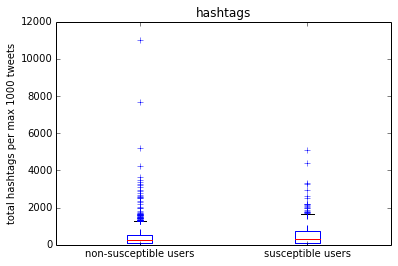
\includegraphics[width=3.0in]{total_hashtags_boxplot}
  \caption{Boxplot for metric: total hashtags}
  \label{fig:hashtags_boxplot}
\end{figure}
This is confirmed on the boxplot.\\\\

\begin{table}[ht!]
\begin{tabular}{llllll}
\textbf{}       & Mean     & Median & Std. Dev  & Lower Q. & Upper Q. \\
Non-susceptible & 2631.046 & 140.5  & 42591.170 & 35.75  & 447.75     \\
Susceptible     & 856.482  & 112    & 4899.689  & 32.5     &  275    
\end{tabular}
\caption{Statistics for total number of incoming favorited (favorite count) tweets for latest tweets (up to a max of 1000)}
\end{table}

The statistics for number of favorited tweets show a larger mean, median and upper quantile for the non-susceptible group. However the standard deviation is also an order of magnitude higher for the non-susceptible group, so this could indicate one or more outliers, especially in the non-susceptible group.
\begin{figure}[H]
  \centering
  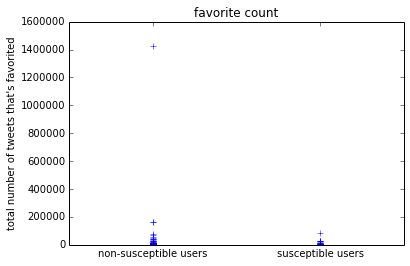
\includegraphics[width=3.0in]{favorite_boxplot}
  \caption{Boxplot for metric: number of favorites}
  \label{fig:favorite_boxplot}
\end{figure}
We see on the boxplot that there is a gross outlier for the non-susceptible users.\\\\
\begin{table}[ht!]

\begin{tabular}{llllll}
\textbf{}       & Mean    & Median & Std. Dev & Lower Q. & Upper Q. \\
Non-susceptible & 318.712 & 206    & 312.943  & 60       &  524.25  \\
Susceptible     & 314.652 & 196    & 301.290  & 66       &   543  
\end{tabular}
\caption{Statistics for total number of urls for latest tweets (up to a max of 1000)}
\end{table}

The statistics for number of urls are very similar and not much can be concluded other than they most likely are not very different from one group to the other.
\begin{figure}[H]
  \centering
  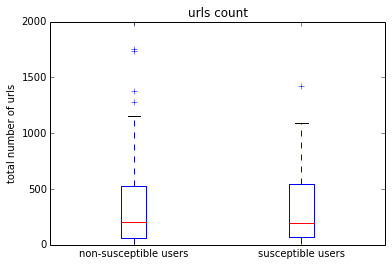
\includegraphics[width=3.0in]{total_urls_boxplot}
  \caption{Boxplot for metric: total urls}
  \label{fig:total_urls_boxplot}
\end{figure}
The similarity is also expressed in the boxplot.
\begin{table}[ht!]

\begin{tabular}{llllll}
\textbf{}       & Mean       & Median  & Std. Dev    & Lower Q. & Upper Q. \\
Non-susceptible & 211963.458 & 14833.5 & 794069.88   & 1794.25    & 94021  \\
Susceptible     & 296314.418 & 25401   & 1412893.447 & 3261.5   &  118909 
\end{tabular}
\caption{Statistics for total number of incoming retweets (retweet count) on latest tweets (up to a max of 1000)}
\end{table}
The mean and median are higher for the susceptible group, but both groups have large standard deviations, where the deviation for the susceptible group is especially large, which indicates outliers in both groups, especially for the susceptible group.
\begin{figure}[H]
  \centering
  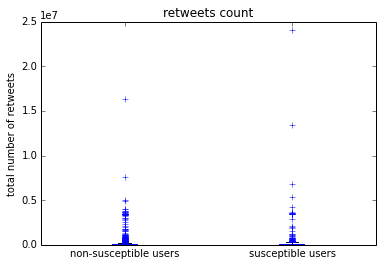
\includegraphics[width=3.0in]{retweets_boxplot}
  \caption{Boxplot for metric: retweets}
  \label{fig:retweets_boxplot}
\end{figure}
The boxplot reveals outliers especially among the susceptible users.
\\\\

In comparing the data between the two groups, we will use a Welch t-test for testing populations with unequal variances to test the null hypothesis that they have equal means or the alternative hypothesis that there is a difference in means of the two groups.
We choose a treshold of 5\% (0.05).
\begin{table}[H]
\centering
\begin{tabular}{lllll}
\hline
Metric & Reciprocal & Non-reciprocal & t-value & p-value \\ \hline
Age & 1204.629 & 1456.636 & 6.290 & 4.952e-10\\
Friends & 9638.393 & 10919.615 & -0.445 & 0.649 \\
Followers & 13369.934 & 61028.298 & -1.107 & 0.268 \\
Hashtags & 531.755 & 422.087 & -3.329 & 0.0009 \\
Urls & 314.652 & 318.712 & 0.246 & 0.805 \\
Statuses & 10627.834 & 11073.442 & -0.374 & 0.707 \\
Retweeted tweets & 296314.418 & 211963.458 & -1.236 & 0.216 \\
Favorited tweets & 856.482 & 2631.046 & 1.396 & 0.162 \\ \hline
\end{tabular}
\caption{The table above shows the mean of each metric for the susceptible users and non-susceptible users. The hashtags metric are hashtags used for a maximum of 1000 tweets. The retweeted tweets metric are the total number of times the users tweets have been retweeted for a maximum of 1000 tweets. The favorited tweets metric are the total number of times the users tweets have been favorited for a maximum of 1000 tweets. The age of account is specified in days.}
\end{table}
We find that for the age of account and the number of hashtags, the null hypothesis can be rejected with our threshold, and thus the alternative hypothesis must be accepted that the means are significantly different from each other.\\

\subsection{Machine-learning - supervised learning}
We trained a Logistic Regression classifier on our data-set with the features specified in the Statistics section: age of account, number of friends, number of followers, number of total hashtags, number of total urls, number of total statuses, number of retweeted tweets and number of favorited tweets. The classifier achieved a consistent accuracy of around 70\% which is the same accuracy percentage as predicting all outputs to be the largest class in our data-set (the non-susceptible class), thus for our data-set with our chosen number of features, it was not very effective.  
\subsection{Network}
We wanted to see if there were a difference between the networks of the two groups. To do this, we would use following methods:\\
\begin{itemize}
  \item Average shortest path
  \item Degree (average degree and degree distribution)
  \item Clustering coefficient
  \item Betweenness centrality \\
\end{itemize}
 There was multiple solutions to fetch the networks, depending on how we defined the network for a group. \\
The first solutions was to fetch all (or a big amount) of each users followers in the group. This idea was quickly dropped do to the Twitter API rate limit. It would simply take forever. \\
In the beginning we were concerned about the proportion which wasn't connected to others in the network. We knew we couldn't avoid this, but maybe we could minimize it. Therefore, the second solution was to find all of the users in first indent (of the group) where minimum one of the users followed the other. This could minimize the non-connected nodes. In the other hand, we could see we manipulated the data which was a no go. \\
The final solution which we ended up with, was to take 30 of the users in each group randomly chosen as well as 100 of their followers and constructing a network graph from that data. \\

As we still ended up with a network not entirely connected, we couldn't calculate the average shortest path and clustering coefficient as it was. But we found a solution to this: Giant component. \\
A giant component is the largest sub-graph of the super-graph where all of the nodes is connected. \\
This could perhaps help us to investigate the two networks further. \\

With help of Networkx\cite{networkx} we found the Giant components of the two groups and with Gephi\cite{gephi} could we visualize them - Figure \ref{fig:giant_comp_non_sus} and \ref{fig:giant_comp_sus}.

\begin{figure}[H]
  \centering
  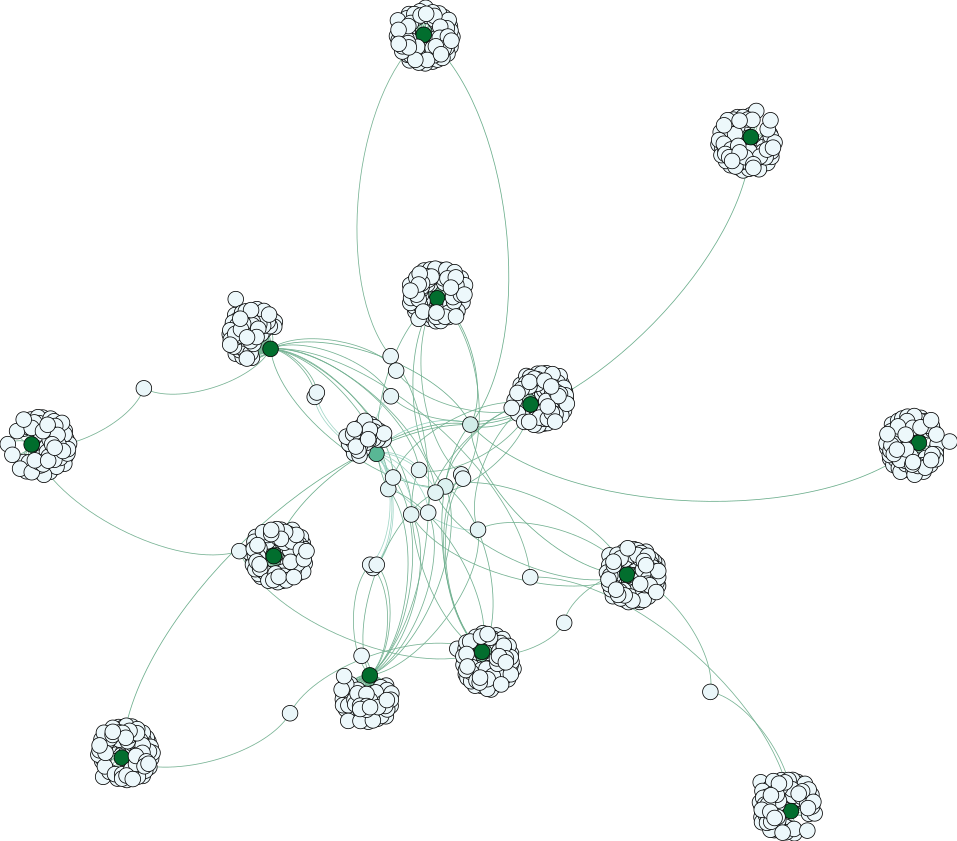
\includegraphics[width=3.0in]{non_rec_giant_component}
  \caption{Giant component of non-susceptible group}
  \label{fig:giant_comp_non_sus}
\end{figure}


\begin{figure}[H]
  \centering
  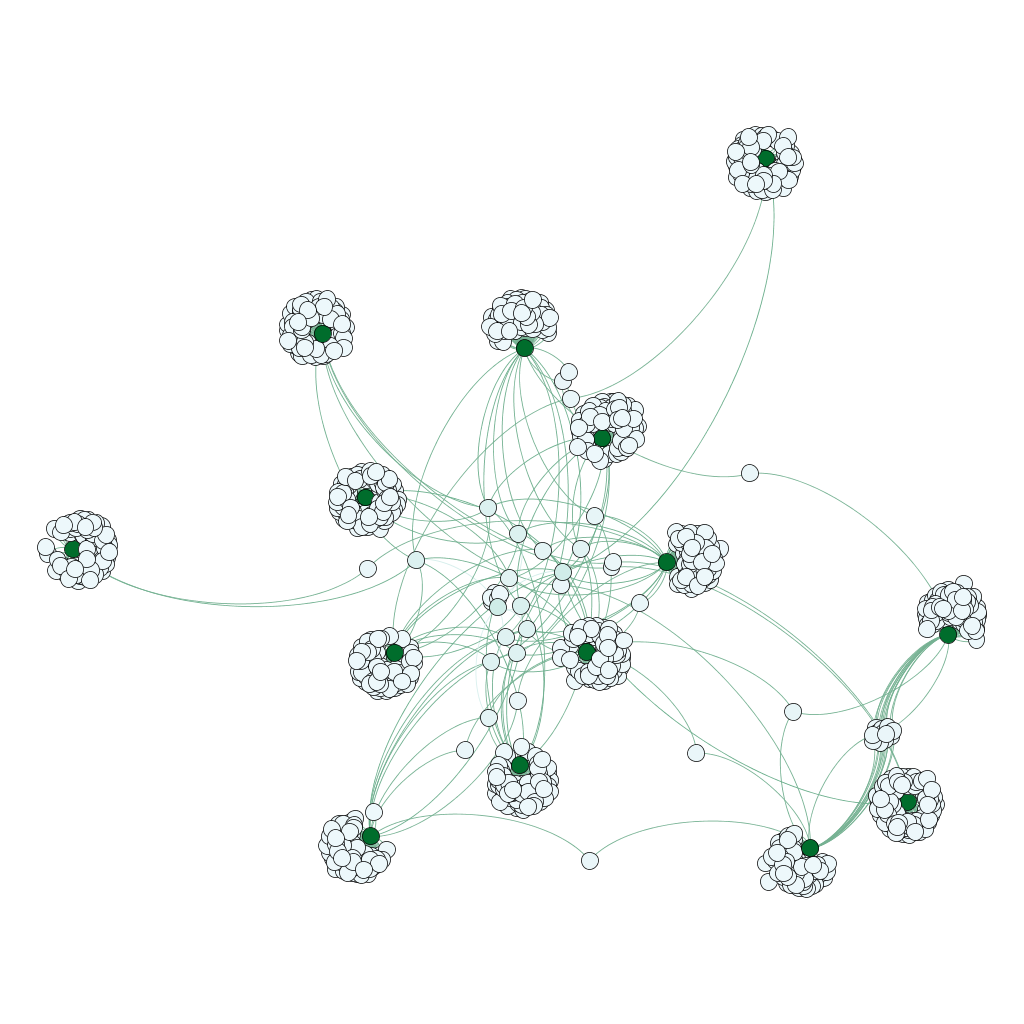
\includegraphics[width=3.0in]{rec_giant_component}
  \caption{Giant component of susceptible group}
  \label{fig:giant_comp_sus}
\end{figure} 

\subsubsection{Average shortest path and average degree}
We we can see from Table \ref{tab:networkKeyNumbers} that here are no special difference between the two groups.  Both average shortest path and average degree is approx. the same.


\begin{table}[H]
\centering
\begin{tabular}{lcc}
\hline
                      & Susceptible & Non-susceptible \\ \hline
No. of nodes          & 1326        & 1318            \\
No. of edges          & 1412        & 1358            \\
Average shortest path length & 4.3363      & 4.3516          \\
Average degree        & 2.127       & 2.061           \\ \hline
\end{tabular}
\caption{Statistics for the networks of the Giant components}
\label{tab:networkKeyNumbers}
\end{table}

If we find the degree distribution for the groups, and plot them (Figure \ref{fig:degree_distribution}), we can that the are almost identically. 
\begin{figure}[H]
  \centering
  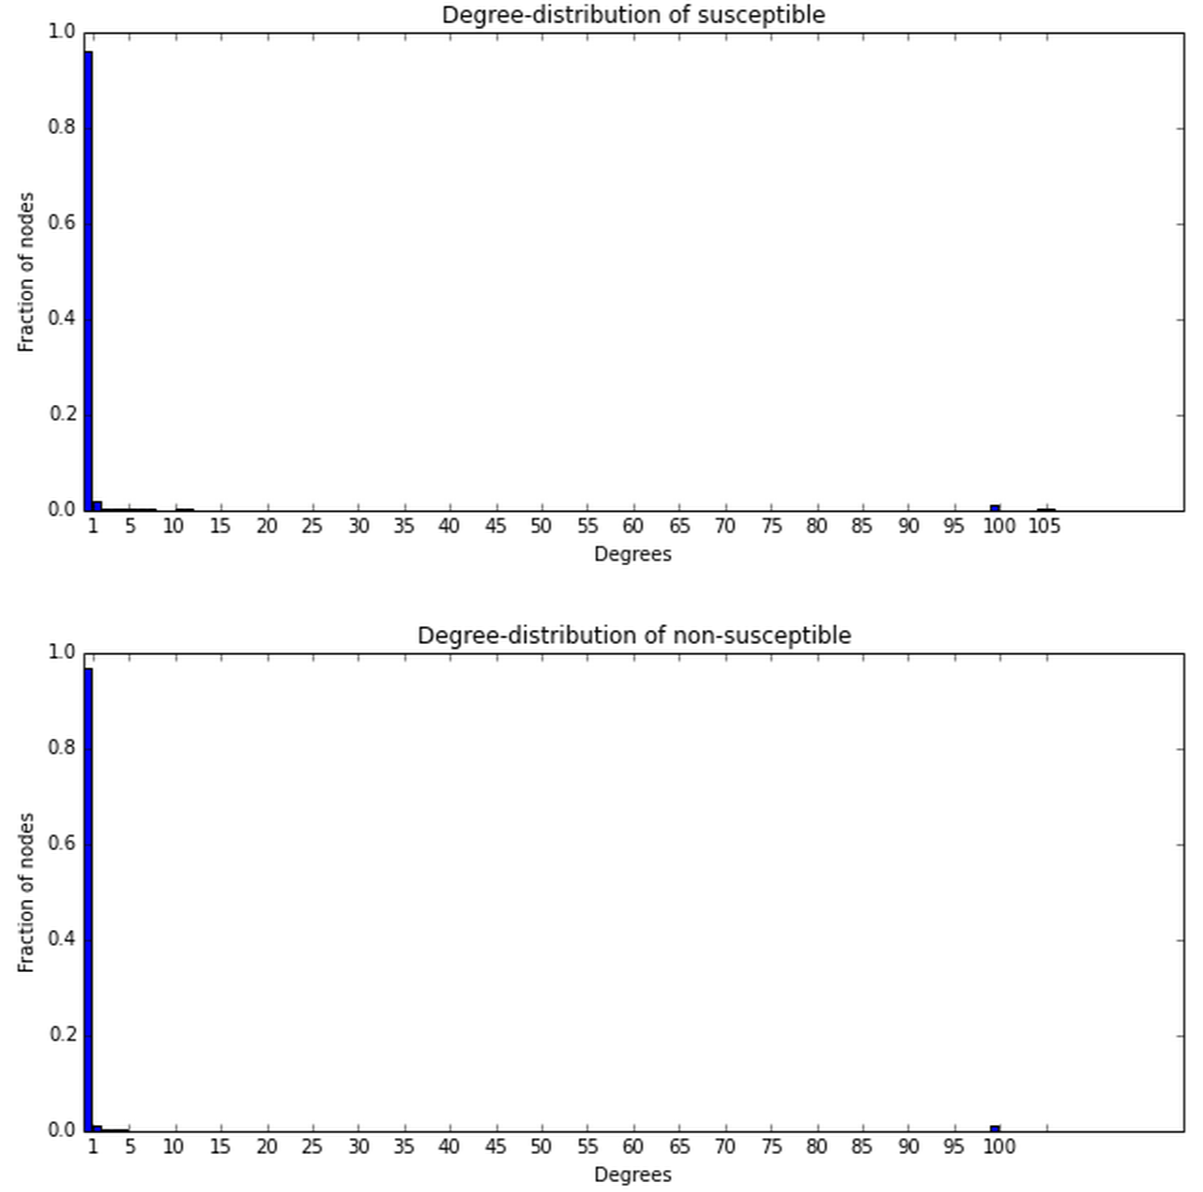
\includegraphics[width=3.0in]{degree_distribution}
  \caption{Degree distribution for the two groups}
  \label{fig:degree_distribution}
\end{figure}


\subsubsection{Clustering coefficient}
We calculated the global clustering coefficient of the groups. At non-susceptible, it gave 0.0. At susceptible it gave a very small number: 0.0002516.\\

This means that with non-susceptible there are 0\% chance for a nodes neighbours also are connected. 
With susceptible there are approx. 0.02516\% chance for a nodes neighbours also are connected. \\
If we look at the maximum local clustering coefficient, the non-susceptible has a maximum of 0.0, while the susceptible has a maximum of 0.3333. \\
Table \ref{tab:clustering_coefficient} summarize this. 
\begin{table}[H]
\centering
\begin{tabular}{lcc}
\hline
                      & Susceptible & Non-susceptible \\ \hline
Global clustering coefficient & 0.0002516 & 0.0           \\
Maximum local clustering coefficient          & 0.3333        & 0.0     \\ \hline
\end{tabular}
\caption{Clustering coefficients of the groups}
\label{tab:clustering_coefficient}
\end{table}

By this there seems to be a difference between the groups by comparing the clustering coefficients. \\

\subsubsection{Betweenness centrality}
We want see if there was a difference between the centrality in the networks, where we used betweenness centrality as a measure. Betweenness centrality of a node is equal to the number of shortest paths from all nodes to all other that pass through that node\cite{betweenness}. \\
So the higher betweenness a node has, the more influence has the node on the network. 
In our case this corresponds to a user is very indirected connected to many others in the network. 
\begin{figure}[H]
  \centering
  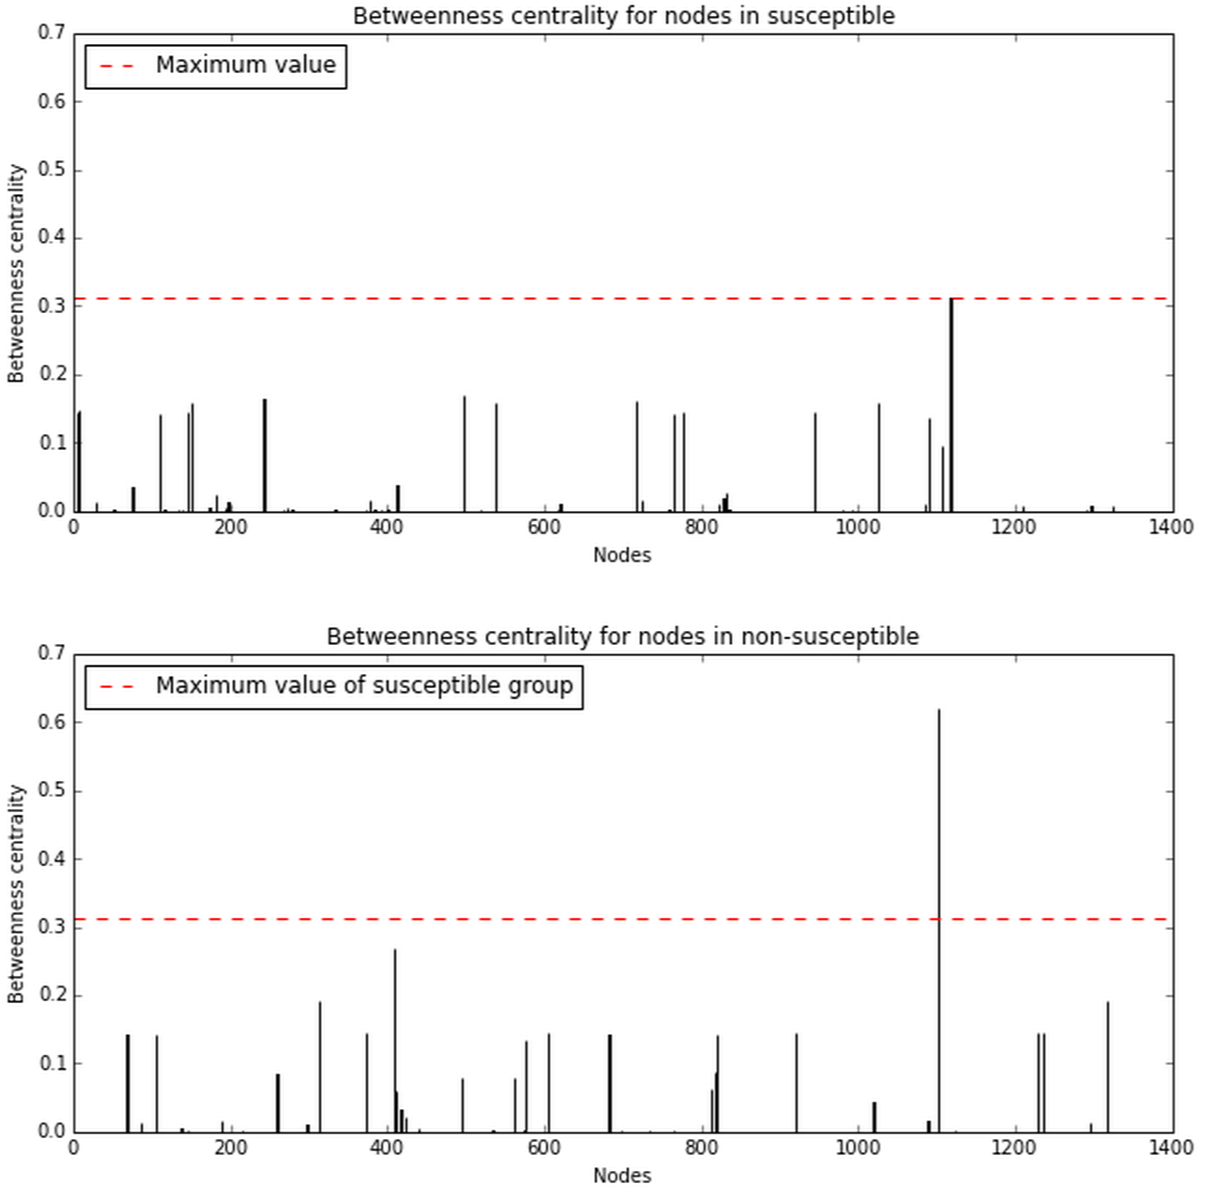
\includegraphics[width=3.0in]{betweenness_centrality}
  \caption{Betweenness centrality for nodes in the groups}
  \label{fig:betweenness_centrality}
\end{figure}
The betweenness centrality is visualized in Figure \ref{fig:betweenness_centrality}. We an compare the two groups by looking on how big the values are and how many of the high values the groups have. \\
We can see that non-susceptible has a node with a very big value around 0.6, where non-susceptible has a maximum around 0.3 (illustrated by the red, dashed line). 
The other nodes in susceptible seems to be a bit lower in general compared to non-susceptible. But to be sure it has to be analysed further. 


\subsection{Sentiment analysis}
We wanted to see if one of the groups was more positive than the other. We used machine learning, by building a classifier based on a corpus. The classifier was based on a simple Naive Bayes and the corpus was based on 13333 positive and negative tweets (26666 tweets total). \\
As both of the groups was relative large, we only classified up to the first 50 tweets per user. Some of the users haven't 50 tweet, so we just classified all tweets. 
Table \ref{tab:sentimentKeyNumbers} show the ratios of the analysis. 

\begin{table}[H]
\centering
\begin{tabular}{lll}
\hline
                       & Susceptible & Non-susceptible \\ \hline
No. of users           & 487         & 1160   \\
No. of tweets          & 23785       & 56097   \\
No. of positive tweets & 14870       & 33468   \\
No. of negative tweets & 8915        & 22629   \\ \hline
\end{tabular}
\caption{Ratios of the sentiment analysis}
\label{tab:sentimentKeyNumbers}
\end{table}

Every of the classified tweets for each user, got either a 0 (negative) or 1 (positive). We then made an overall verdict for each user based on normalized positives and negatives, and a majority voting system, so the verdict could be one of the following:

\begin{itemize}
  \item Strong negative
  \item Slight negative
  \item Neutral
  \item Slight positive
  \item Strong positive\\
\end{itemize}

As we wanted to compare the groups, we compared an equal large population of them. As susceptible was smaller, we chose 487 of the non-susceptible group, so the both was 487.  \\

\begin{figure}[H]
  \centering
  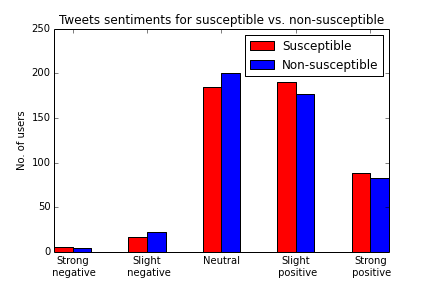
\includegraphics[width=3.0in]{sentiment_barplot}
  \caption{Sentiment distribution between the two groups}
  \label{fig:sentiment_barplot}
\end{figure}


As we can see from the result, there are really no particularly differences between the groups. Though from the figure in this example, we can see that the susceptible is generally more positive than the non-susceptible. But to generalize this, will be a very weak assumption. 

\subsection{Theory}
We have used several of the tools learned in the course for the report, below is a list of tools we have used.\\
\subsubsection{Machine learning}
We have used machine learning to try to classify non-susceptible users from susceptible users. We used the dataset the bot has accumulated over the duration of the course with a Logistic Regression classifier. However we found with our selected features, classifier and data-set we were not successful in classifying above simply predicting the largest class in the data-set.\\
\subsubsection{Network Theory}
In network theory have we used average shortest path length, average degree and degree distribution, clustering coefficient and betweenness centrality. \\
\subsubsection{Natural Language Processing}
We have used NLP to find the sentiment of the users tweets, so we could tell if the user generally writes positive or negative.\\
We used an self-made corpus and som machine learning tools. \\
\subsubsection{Python and relevant libraries}
For the bot as well as doing the analysis for this report we have relied on Python, its standard library and the external libraries: twitter, nltk, sklearn, requests, beautiful soup, numpy, pymongo, networkx.
\section{Conclusion}

A conclusion can be drawn that creating a human-like bot that can gain a lot of followers and to some degree influence people is possible. The things we would've done differently and our advice to future bot designers is to follow users based on the criteria we found in this report, made users susceptible. The criteria we found for making users susceptible was: Following accounts with a low account age, high number of hashtags in tweets, and possibly: low number of favorited tweets, high friend count, high number of retweet tweets.\\\\

We would also advise creating and posting content early to picque potential subsceptible users interest, and utilizing website scraping for content generation, as we noticed it helped the bot generate more followers.

\bibliographystyle{IEEEtran}
\bibliography{lyngby}
\begin{thebibliography}{9}

\bibitem{twitterprofile}
\url{twitter.com/JackBoHorseMan}
\textit{JackBoHorseMan Twitter Profile}

\bibitem{networkx}
\url{https://networkx.github.io/}
\textit{Networkx package for Python}

\bibitem{gephi}
\url{http://gephi.github.io/}
\textit{Gephi - network visualization}

\bibitem{betweenness}
\url{http://en.wikipedia.org/wiki/Betweenness_centrality}
\textit{Betweenness centrality - Wikipedia}
\end{thebibliography}

\clearpage
\onecolumn
\appendices
\section{Code listings}

\definecolor{darkgreen}{rgb}{0, 0.4, 0}
\lstset{language=Python,
  numbers=left,
  frame=bottomline,
  basicstyle=\scriptsize,
  identifierstyle=\color{blue},
  keywordstyle=\bfseries,
  commentstyle=\color{darkgreen},
  stringstyle=\color{red},
  literate={Ö}{{\"O}}1 {é}{{\'e}}1 {Å}{{\AA}}1,
}
\lstlistoflistings

\end{document}
